\subsection{Estructura General del Sistema}
El proyecto Packlead está armado con una arquitectura modular, pensada por funcionalidades (screaming architecture). La idea principal es que sea fácil de escalar, que se pueda mantener de tal manera en la que los datos se sincronicen ante cambios de estado en la interfaz o de los servicios.

De esta forma logramos separar muy claro las partes: la lógica del negocio, el manejo de la data, la interfaz que ve el usuario y los servicios más técnicos. Así todo fluye de manera ordenada y sin que se arme lío en el sistema logístico. A continuación, se presentan los principales componentes estructurales del proyecto:

\begin{itemize}
    \item \textbf{lib/core:} Configuración global, modelos de datos compartidos y utilidades para mapas, variables de entorno y elementos base del sistema.
    \item \textbf{lib/features/admin:} Módulo administrativo encargado del monitoreo logístico, dashboard de indicadores y visualización en tiempo real de repartidores y pedidos.
    \item \textbf{lib/features/dispatcher:} Módulo operativo del repartidor que gestiona la captura de ubicación GPS, rutas asignadas y actualización de estados de entrega.
    \item \textbf{lib/features/orders:} Capa de datos que implementa el patrón Repository para la sincronización de pedidos con Firebase Realtime Database.
    \item \textbf{lib/navigation:} Sistema de enrutamiento que controla el flujo de la aplicación según el rol del usuario (administrador o repartidor).
    \item \textbf{lib/services:} Servicios técnicos para la integración con Firebase, APIs externas y acceso a geolocalización del dispositivo.
\end{itemize}

\begin{figure}[H]
    \centering
    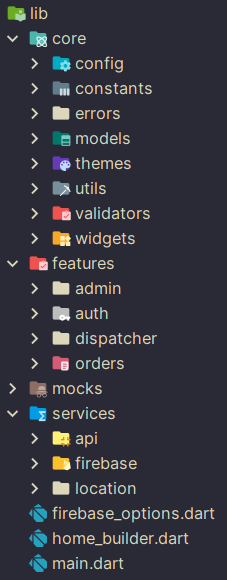
\includegraphics[width=1 \textwidth, height=15cm, keepaspectratio]{img/Estructura.png}
    \caption{Estructura}
    \label{fig:estructura1}
\end{figure}

\subsection{Sistema de Sincronización y Persistencia}
La parte que se encarga de los datos en el sistema usa el patrón Repository. Básicamente, esto sirve para que toda la lógica de cómo hablamos con la base de datos quede separada del resto de la aplicación. Así no se mezcla todo y es mucho más fácil mantener el código, hacer pruebas y después escalar el proyecto si hace falta. La clase que hace todo este trabajo es OrderRepositoryImp, que funciona como el puente entre la app y Firebase Realtime Database.

Cuando se cambia el estado de un pedido, no solo se escribe una palabra o un texto cualquiera. El sistema actualiza el estado actual y también guarda la fecha y hora exacta en que se hizo el cambio. Esto se hace con actualizaciones parciales en la base de datos, o sea, solo se toca lo que realmente cambió y no se reescribe todo el registro de una vez. Como Firebase tiene sincronización en tiempo real, cualquier modificación aparece al instante en todos los dispositivos que estén conectados: el admin, el repartidor y el cliente siempre ven la información actualizada sin tener que refrescar nada.
\begin{lstlisting}
@override
Future<void> updateOrderState(String orderId, OrderState newState) async {
  try {
    // Referencia al nodo específico del pedido en Firebase para una actualización parcial
    await _database.child('orders/$orderId').update({
      'state': newState.name,
      'updatedAt': DateTime.now().toIso8601String(),
    });
  } catch (e) {
    throw Exception('Error al actualizar el estado del pedido: $e');
  }
}
\end{lstlisting}

\subsection{Motor de Rastreo y Geolocalización Dinámica}
El sistema de rastreo es la parte más importante de la app, ya que nos permite ver en tiempo real dónde está cada repartidor. Para eso usamos el plugin Geolocator, que obtiene las coordenadas GPS del celular con la máxima precisión posible. Estas coordenadas se capturan cada cierto intervalo y las manejamos con un provider de estado reactivo que se encarga de toda la información del repartidor.

El proceso va en dos pasos: primero, la ubicación se actualiza directamente en el dispositivo para que el repartidor vea su posición actual en la interfaz sin ningún retraso. Luego, esa misma información se envía y se sincroniza con la base de datos en la nube. De esta forma, los administradores pueden ver en el mapa la ubicación exacta de cada repartidor en tiempo real.

Con este sistema se logra seguir las entregas que están en curso, ajustar rutas cuando sea necesario y mejorar la eficiencia general sin tener que estar preguntando manualmente todo el tiempo dónde se encuentra cada persona.
\begin{lstlisting}
Future<void> updateCurrentLocation() async {
  // Obtención de coordenadas actuales del GPS con alta precisión
  final position = await Geolocator.getCurrentPosition(
    desiredAccuracy: LocationAccuracy.high
  );
  
  // Actualización del estado local y notificación a la UI
  state = state.copyWith(
    currentLocation: Location(
      latitude: position.latitude,
      longitude: position.longitude,
    ),
  );
  
  // Sincronización con el repositorio para que el Admin lo vea en el mapa
  await _repository.updateLocation(state.id, state.currentLocation!);
}
\end{lstlisting}

\subsection{Dashboard de Analítica y Modelado de Datos}
El panel de administración usa una capa intermedia que se llama ViewModel. Básicamente, este ViewModel se encarga de preparar y organizar toda la información antes de mostrarla en la pantalla. En concreto, el AdminOrdersViewModel junta los datos de los pedidos, los repartidores y las ubicaciones para crear un modelo mucho más limpio y rápido que se pueda usar en gráficos, indicadores y reportes.

De esta manera, la interfaz no tiene que hacer cálculos pesados y todo fluye mejor. Así se pueden armar dashboards dinámicos que muestren los KPIs importantes, el estado actual de los pedidos y otras métricas de operación. Al final, los administradores ven en tiempo real cómo va todo el tema logístico y pueden tomar decisiones rápidas y bien informadas para que la distribución funcione más eficiente.
\begin{lstlisting}
// Cuando obtenemos un Order, construimos el AdminOrderVM (añadiendo datos extra del repartidor)
factory AdminOrdersViewModel.fromOrder(Order order, Dispatcher? dispatcher) {
  return AdminOrdersViewModel(
    id: order.id,
    clientName: order.clientName,
    clientPhoneNumber: order.clientPhoneNumber,
    location: order.location,
    address: order.address,
    state: order.state,
    zone: order.zone,
    deliveryDate: order.deliveryDate,
    createdAt: order.createdAt,
    dispatcherId: order.dispatcherId,
    dispatcherName: dispatcher?.name,
  );
}
\end{lstlisting}

\subsection{Arquitectura de Navegación por Roles}
La app tiene un sistema de navegación que depende del rol del usuario, sobre todo diferencia entre administradores y repartidores. Cuando alguien se loguea, el enrutador principal mira qué tipo de cuenta es y lo lleva directo a la pantalla que le corresponde. Así cada persona solo ve y usa las partes que realmente necesita para su trabajo, lo que hace que sea más seguro y también más cómodo de usar.

Para los administradores, la interfaz está pensada para ver todo el panorama de la logística, monitorear cómo va la operación y revisar datos y análisis. En cambio, los repartidores entran a una sección más enfocada: ver las rutas que les tocaron, seguir su entrega en tiempo real y actualizar el estado de los pedidos. De esta forma se evita que la pantalla se llene de cosas innecesarias, se reduce la confusión y nadie accede a información que no le toca ver.
\begin{lstlisting}
static Route<dynamic> generateRoute(RouteSettings settings) {
  final role = MockAuthService.currentRole;

  Route<dynamic>? route;

  if (role == UserRole.admin) {
    route = AdminRouter.generateRoute(settings);
  }

  if (role == UserRole.dispatcher) {
    route = DispatcherRouter.generateRoute(settings);
  }

  return route ?? AuthRouter.generateRoute(settings);
}
\end{lstlisting}

\subsection{Automatización de Infraestructura y Configuración}
El proyecto tiene un sistema automático para crear los archivos de configuración que necesita para conectarse a servicios externos como Firebase y Google. Todo esto lo manejan unos scripts escritos en Dart que leen las variables de entorno desde un archivo .env. Así se mantienen seguras las claves y contraseñas importantes, y se evita tener que configurar todo a mano (que siempre termina saliendo mal en algún momento).

Gracias a esta automatización, es mucho más fácil pasar el proyecto de un entorno a otro: desarrollo, pruebas o producción, sin que se arme un desastre con las configuraciones diferentes. Todo queda consistente y el despliegue se hace más rápido, más seguro y se puede repetir sin problemas cada vez que sea necesario. Esto es clave cuando la app depende tanto de servicios en la nube.
\begin{lstlisting}
Future<void> main() async {
  // Verificación de existencia del archivo de variables de entorno
  if (!File('.env').existsSync()) {
    print('Error: .env file not found');
    exit(1);
  }

  print(' Generating configuration files...\n');

  // Ejecución del proceso para generar google-services.json de forma segura
  final googleServicesResult = await Process.run(
    'dart',
    ['scripts/generate_google_services_json.dart'],
    environment: {...Platform.environment, ...envVars},
  );

  // Ejecución del proceso para generar firebase.json integrando servicios en la nube
  final firebaseJsonResult = await Process.run(
    'dart',
    ['scripts/generate_firebase_json.dart'],
    environment: {...Platform.environment, ...envVars},
  );
}
\end{lstlisting}

\subsection{Ejecución}
La aplicación inicia cargando configuraciones, conectándose a Firebase y activando los módulos principales. Posteriormente, sincroniza datos en tiempo real para monitorear pedidos, ubicaciones y estados logísticos.

\begin{figure}[H]
    \centering
    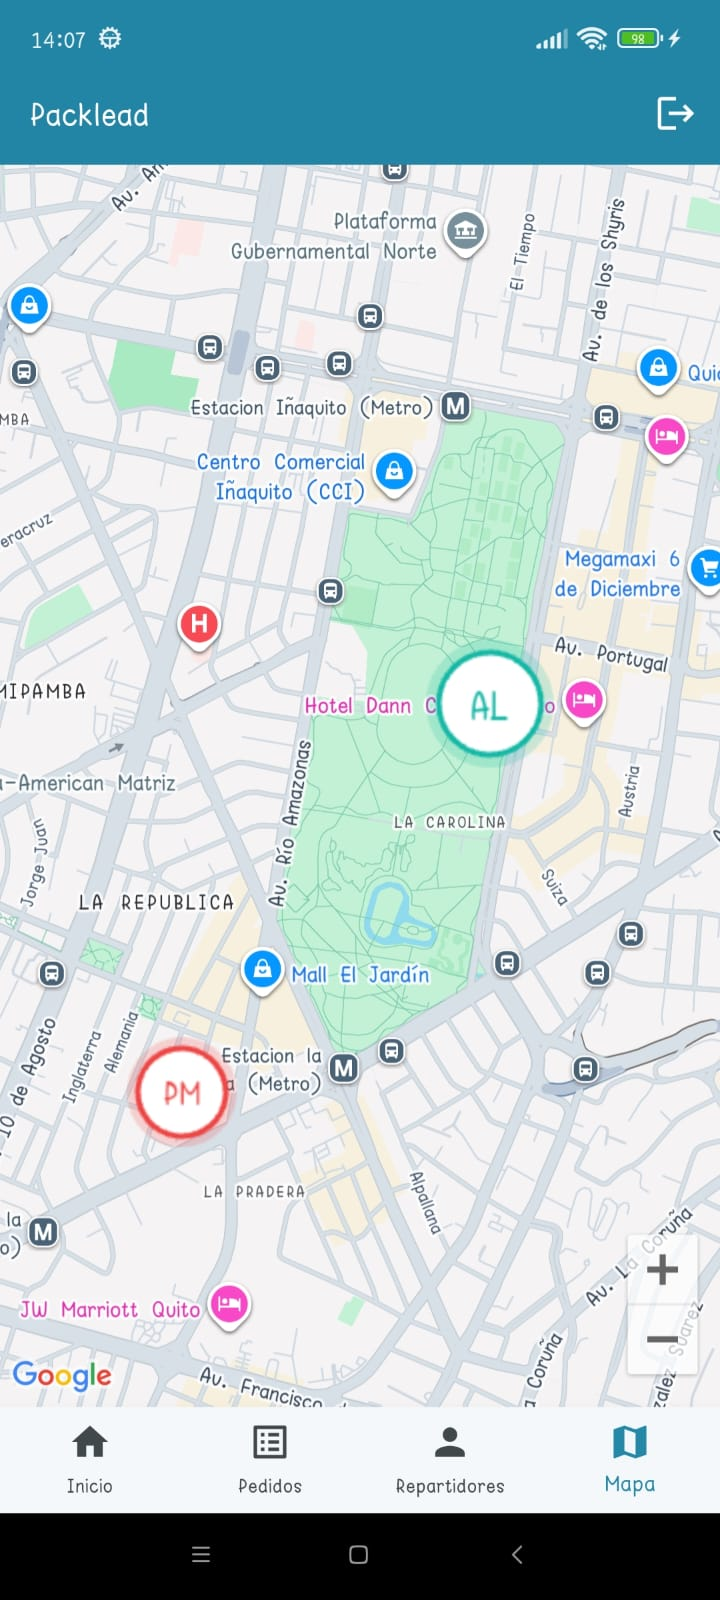
\includegraphics[width=0.8 \textwidth, height=10cm, keepaspectratio]{img/App.jpeg}
    \caption{Mapa de seguimiento en tiempo real}
    \label{fig:irt_map}
\end{figure}